\documentclass{article}
\usepackage[utf8]{inputenc}
\usepackage{tikz}
\usetikzlibrary{shapes, arrows.meta, positioning}

\begin{document}

\begin{figure}[htbp]
\centering
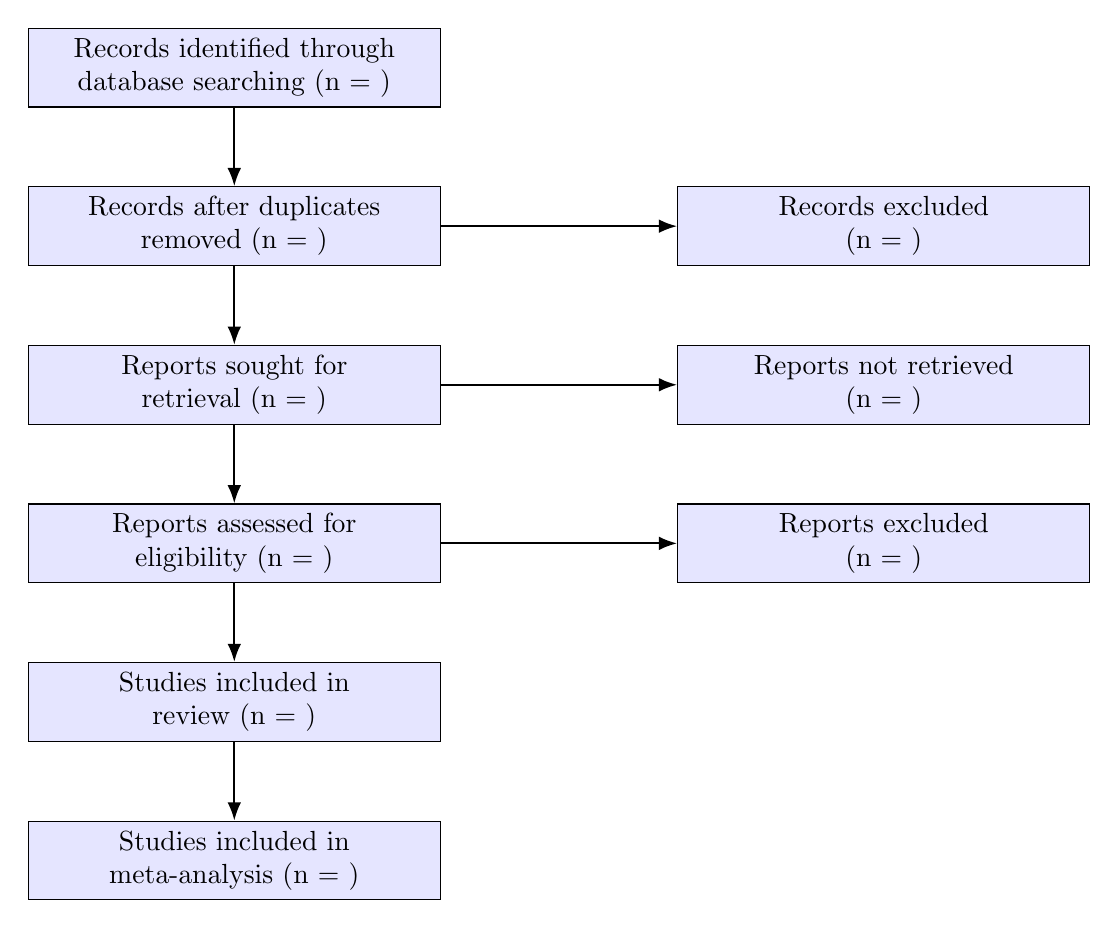
\begin{tikzpicture}[
    node distance=1cm,
    box/.style={rectangle, draw, text width=5cm, text centered, minimum height=1cm, fill=blue!10},
    arrow/.style={-Latex, thick}
]

% Identification
\node[box] (identification) {Records identified through\\database searching (n = )};

% Screening
\node[box, below=of identification] (screening) {Records after duplicates\\removed (n = )};

\node[box, right=3cm of screening] (excluded1) {Records excluded\\(n = )};

% Eligibility
\node[box, below=of screening] (eligibility) {Reports sought for\\retrieval (n = )};

\node[box, right=3cm of eligibility] (excluded2) {Reports not retrieved\\(n = )};

\node[box, below=of eligibility] (assessed) {Reports assessed for\\eligibility (n = )};

\node[box, right=3cm of assessed] (excluded3) {Reports excluded\\(n = )};

% Included
\node[box, below=of assessed] (included) {Studies included in\\review (n = )};

\node[box, below=of included] (meta) {Studies included in\\meta-analysis (n = )};

% Arrows
\draw[arrow] (identification) -- (screening);
\draw[arrow] (screening) -- (excluded1);
\draw[arrow] (screening) -- (eligibility);
\draw[arrow] (eligibility) -- (excluded2);
\draw[arrow] (eligibility) -- (assessed);
\draw[arrow] (assessed) -- (excluded3);
\draw[arrow] (assessed) -- (included);
\draw[arrow] (included) -- (meta);

\end{tikzpicture}
\caption{PRISMA 2020 Flow Diagram}
\label{fig:prisma}
\end{figure}

\end{document}
